\documentclass{beamer}
\usepackage[utf8]{inputenc}
\usepackage[T1]{fontenc}
\usepackage[french]{babel}
\usepackage{graphicx}
\usetheme{Warsaw}


\begin{document}

\title{Projet Pire2Pire}
\author {
CLERIS Audrey        \\
MARZIN Amélie        \\
REPAIN Alex          \\
ROBERT Valentin      \\
ROELANDT Cyril
}


\begin{frame}
    \titlepage
\end{frame}

\begin{frame}
    \section{Caractéristiques}
    \begin{itemize}
        \item Compatible GNU/Linux (Debian/Ubuntu) et *BSD (FreeBSD)
        \item Probablement compilable avec n'importe quel compilateur
        \begin{itemize}
            \item ... avec une libc sans extension GCC...
        \end{itemize}
        \item Démon Unix
        \item Application multi-threadée
        \item Presque sans memory leaks !
    \end{itemize}
\end{frame}

\begin{frame}
    \section{Pool thread}
    \begin{itemize}
        \item N threads crées au démarrage du démon
        \item Dorment en attendant des jobs
        \item Jobs "rapides" et jobs "lents"
    \end{itemize}
\end{frame}

\begin{frame}
    \section{Clients et démons}
     \textbf{Le client}

    \begin{itemize}
        \item Interagir avec l'utilisateur humain
        \item Fonctionnement : 
            \begin{itemize}
                \item Envoyer les commandes tapées au démon
                \item Renvoyer les réponses à l'utilisateur
            \end{itemize}
    \end{itemize}
\begin{center}
\begin{figure}[htbp]
    \centering
    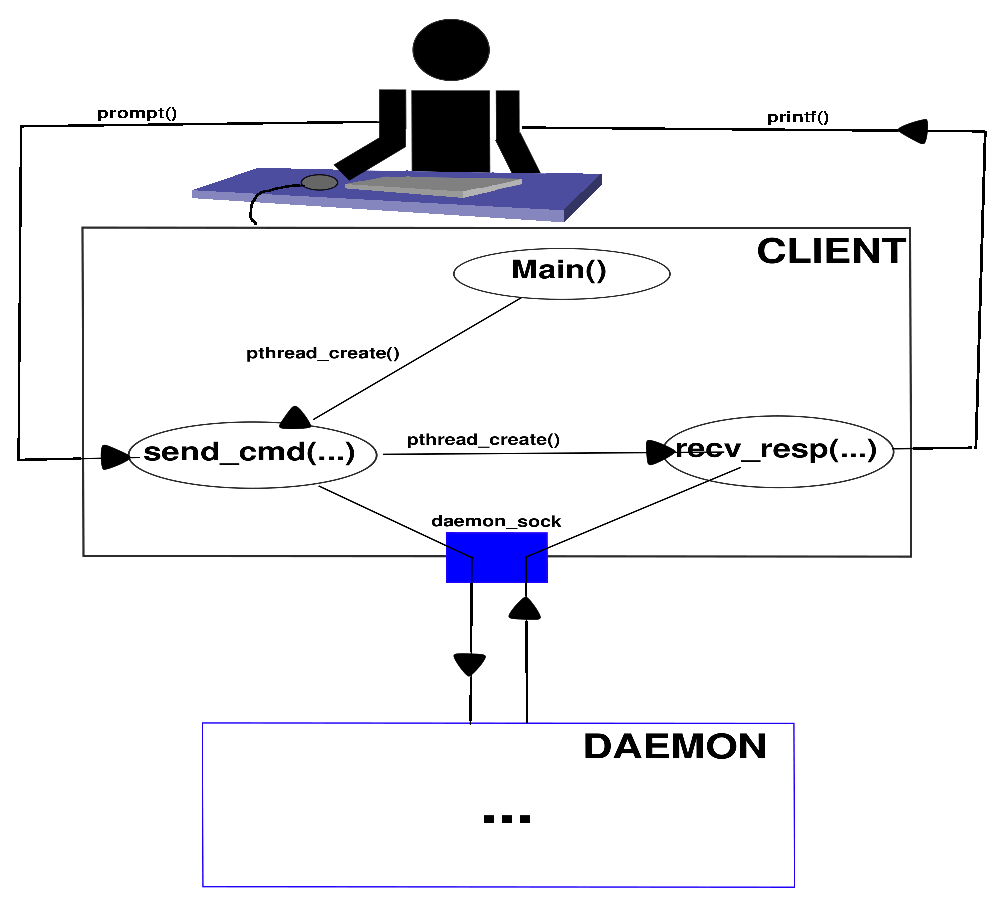
\includegraphics[scale=0.8]{archi_client.eps}
\end{figure}
\end{center}


\end{frame}

\begin{frame}
    \textbf{Le démon}
    
    \begin{itemize}
        \item Exécution en arrière-plan
        \item Gestion de toutes les requêtes (clients et démons)
        \item Vision globale : liste de clients et démons connus
        \item Utilisation des pool de threads :
            \begin{itemize}
        \item 2 pools pour les clients et les démons
        \item 2 pools pour les requêtes rapides et lentes
            \end{itemize}
    \end{itemize}
\end{frame}

\begin{frame}
    \section{Requêtes}
\end{frame}


\end{document}
